\documentclass[a4paper,11pt]{article}
\usepackage[a4paper, total={6in, 10in}]{geometry}
\usepackage[english]{babel}
\usepackage[utf8]{inputenc}
\usepackage{hyperref}
\usepackage{caption}
\usepackage{subcaption}
\usepackage{siunitx}

\usepackage{float}

\usepackage{graphicx}
\usepackage{latexsym}
\usepackage{multicol}



\hypersetup{
    colorlinks=true,
    linkcolor=blue,
    filecolor=magenta,      
}

\providecommand{\keywords}[1]{\textbf{\textit{Keywords ---}} #1}

\newcommand\FramedBox[3]{%
  \setlength\fboxsep{0pt}
  \fbox{\parbox[t][#1][c]{#2}{\centering\huge #3}}}

\renewcommand{\figurename}{Fig.}
\renewcommand{\tablename}{Tabela}

\DeclareMathSizes{12}{20}{14}{10}

\author{ Camilo Sad  \\
 Carlos Rebelato \\
 Cristina Freitas Bazzano \\
 Professor Jeremy Hajek }
 
\begin{document}

\begin{figure}
\centering
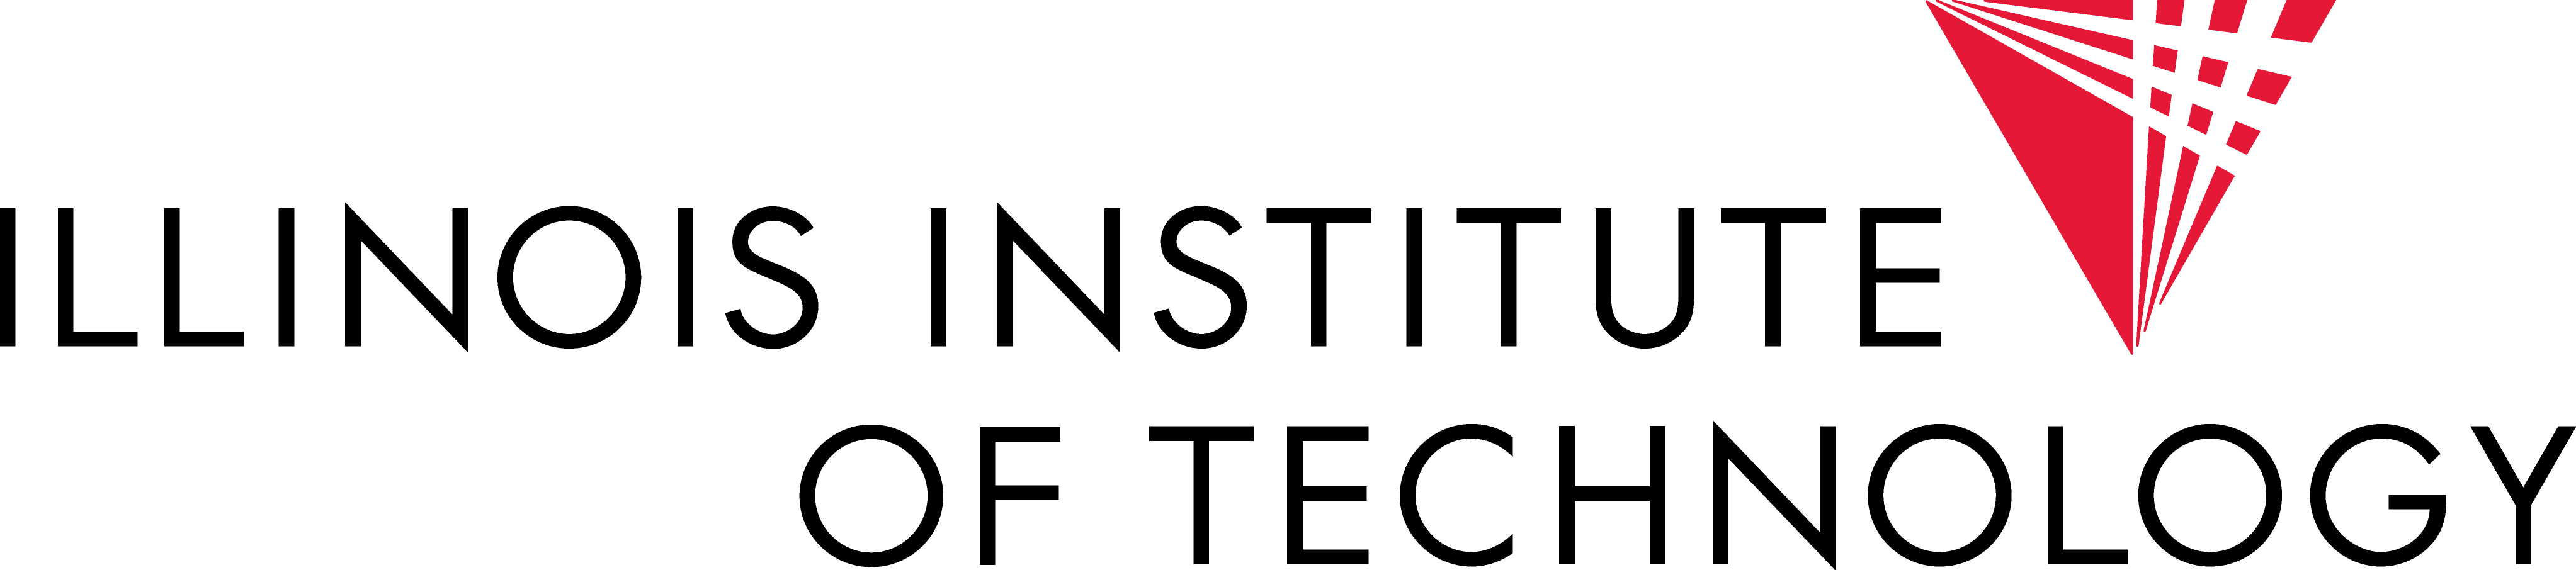
\includegraphics[width = 0.7\linewidth]{images/IIT_Logo_stack_186_blk}
\label{iitlogo}
\end{figure}

\title{Data Analyses and Presentation \\
\large Glass Charts \\
A Google Glass Application}

\maketitle

\begin{figure}[H]
\centering
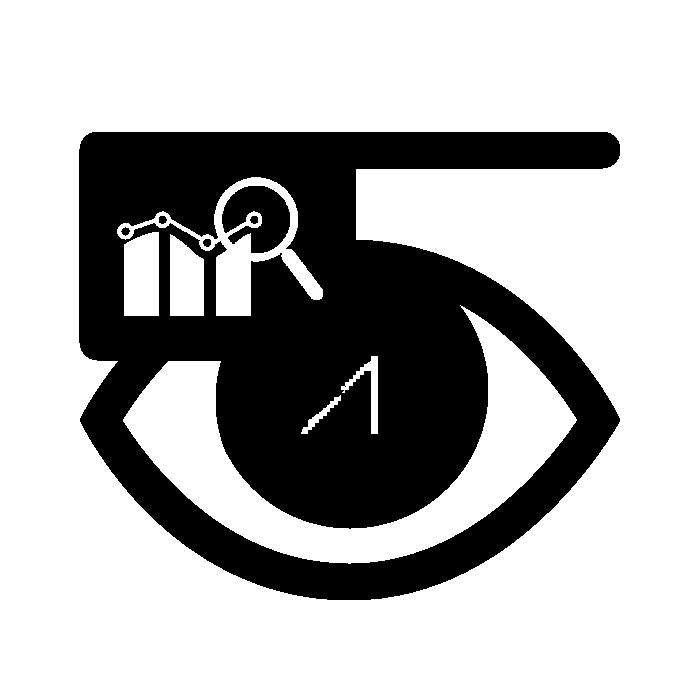
\includegraphics[width = 0.2\linewidth]{images/glass_charts_logo_black.png}
\label{projectlogo}
\end{figure}

\medskip

\begin{abstract}
Technology is something that is in constant development \cite{tecmundoandroid}. Nowadays, we are living in an era where everybody has to deal with it, every single day. The amount of devices that have been built throughout the years cannot be counted and the amount of upcoming projects and studies in this area are also countless. Big companies and scientists have put a lot of effort in this area and they have been successful. A lot of devices have been produced successfully and they have also been improved a lot. The population’s life has been improved a lot with the help of these devices and the technology itself. Simple tasks, day by day chores and even the most complex activities people need to do, everything can be simplified by the use of the right devices.

Google Glass is one of these devices that came to make life easier \cite{googleglassproject}. Projected by Google, this device has, as its main goal, to help users do simple tasks such as calls, check emails and get directions to a specific place. With the objective to help technicians, faculty staff and all the workers that need to access data in an easy way while doing other tasks, this project was developed. A study was made to understand the platform better and also to understand how capable its software and hardware are. Limitations were found, being one of the biggest of them the fact that the platform is really simplistic.
\end{abstract}


\keywords{ Google Glass, Sensors, Internet of Things, Data  Presentation }

\medskip

\section{Introduction}

There are many situations where controlling and monitoring some environment aspects, such as temperature and humidity, is crucial for the quality of the work being executed or even for the safety of the workers. In our project we will help to keep control of environmental data, and to do so we retrieve data from an online server and present it in different charts to highlight the measurements variations.

This project can be applied to different scenarios, and our implementation focus in the refrigeration system control of buildings. The data are measurement of different rooms and it have different time scopes, varying from time of the day through week of the month to month of the year. Our goal is to enable technicians and all interested workers the access to this environmental data while doing other tasks. The use of a compact platform is the key to make this project possible and worth it.

\section{Technologies}

\subsection{Google Glass}

Google Glass is a device that contains an optical display with a touchpad attached to it that has the shape of a pair of eyeglasses \cite{glassdevelopers,tecmundoandroid}. It has as its main goal to be a ubiquitous computer, to be something that is always ready for the user to use without disturbing the user’s activities. 

There are multiple ways for the user to interact with it: as previously mentioned, users can interact with it through the touchpad, as well as giving voice commands, and there’s also some features where you can configure the device to answer actions like the blink of an eye.

Glass is fundamentally different than existing mobile platforms in both design and use. It works best with information that is simple, relevant, and current. It runs with the concept of cards, where each view of the application is a card. These cards must have a simple design, it only accepts text, image, video and HTML. When designing an application for it you have to follow some principles and patterns to be able to deliver the information you want in the best way that the platform can handle. Below is an example of a glassware design.

\begin{figure}[H]
\centering
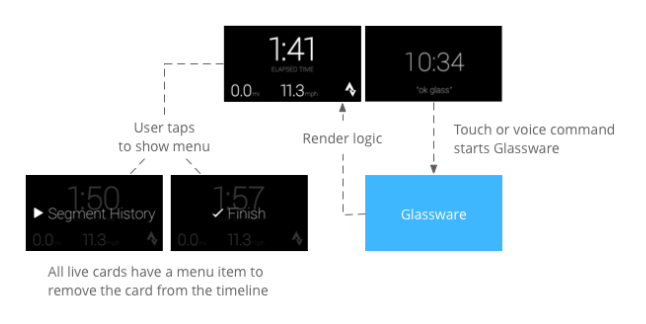
\includegraphics[width = 0.6\linewidth]{images/glass_cards_example.png}
\caption{Glassware Example}
\label{cardexample}
\end{figure}

Google started distributing prototypes \cite{googleglassstyle} in the United States on April 15, 2013, but only to qualified people and each device was costing \$1,500. A little bit later, on May 15, 2014, it became available to the public for the same price as it was sold before.

During its appearance, the headset has received a lot of criticism and legislative actions \cite{glassprivacy} due to privacy and safety concerns and on January 15, 2015 Google announced that the production of the device would be over but that its development would continue.

\subsection{Android}

Android is an operational system \cite{androiddevelopers} based on Linux and nowadays it is developed by Google. It was designed to work mainly with devices with touchscreens. This is the most used mobile operational system over all the world. Android’s source code is provided by Google and runs under the open source license.

To develop to Google Glass a specific development kit is needed, the Glass Development Kit (GDK), which is an add-on to the Android SDK that lets you build Glassware that runs directly on Glass. This development kit works with Android version 4.4.2 running the API 19.

\subsection{AChartEngine}

AChartEngine is a charting library for Android applications \cite{acharengine}. It supports a large amount of chart types, matching all the needs based on the data that is going to be presented.

Charts can contain multiple series and also can be modified and support many other custom features. They can be built as a view that can be added to a view group or a new intent.
Currently the library is on the version number 1.0.0 and the developers affirmed that new features will be added in future releases. 

This technology was used to render charts based on the data retrieved from the database. Whenever the application receives data from the server (at every launch), the answer from the server will be read and turned into a collection of Java objects that will hold the information to feed the charts later.

We used two different chart types in our application, bar charts and line charts, both of them were filled with time data. And we created a render class to be able to model the chart in the best way we could find.

\subsection{Node Server}

A server was needed to implement this project. It has two main functions: to help sensors to persist their data on the database and handle the calls made by the application that is running on Glass in order to retrieve data from the database and build the charts. 

The server runs over a Node.JS environment \cite{herokudev}. Node.js is a JavaScript runtime built on Chrome's V8 JavaScript engine. Node.js uses an event-driven, non-blocking I/O model that makes it lightweight and efficient. Node.js' package ecosystem, npm, is the largest ecosystem of open source libraries in the world.

\subsection{V8 Engine}

V8 is Google's open source high-performance JavaScript engine, written in C++ and used in Google Chrome, the open source browser from Google \cite{v8server}. It implements ECMAScript as specified in ECMA-262, can run standalone, or can be embedded into any C++ application.

\subsection{Mongo Database}

MongoDB is a free and open-source cross-platform database \cite{mongodb}. It’s classified as a NoSQL database, going far away from what the usual databases, such as MySQL, are. It works with dynamic documents through the use of the JSON structure. MongoDB is developed by MongoDB Inc. and runs under the open source license \cite{mongodbdocs}.

\subsection{Heroku}

Being in development since 2007, Heroku is a cloud service that works as a Platform-as-a-Service \cite{heroku}. It provides the customer an environment to develop, run and manage applications without the need of configuring the whole environment from scratch. It helps developers throughout the whole application’s lifetime, since development and deployment until the maintenance cycle. In this project, Heroku was where the NodeJS server and the database were both deployed.

\subsection{Git}

Git is a distributed version control system that emphasizes speed and teamwork \cite{git}. Initially, it was developed to help to build Linux, but it was adopted by other projects.

In this specific project, GitHub was used. GitHub is as web-based Git repository hosting service that offers a lot of revision control and source code control management. 

This technology was essential throughout all the application's development. By using it, we could have control over the Glassware’s code and all the other files that made part of the project, such as texts and presentations. 

\section{Application Overview}

The application built is simple and direct, just as a Glassware should be \cite{glassdevelopers}. It contains a main screen from where the user is directed to access the charts by voice or touch commands to open the main menu. Each type of measurement chart (Temperature, Humidity, and Pressure) have three different scopes within them: hours within a day, weeks within a month, and months within an year. You can navigate among these scopes by using touch commands. From the menu, there is also an option to open an instruction screen that explains to the new users how to use the application.

All the data that is presented within the charts is retrieved from the server. A HTTP call is made to the server as soon as the user opens the application and then it is shared among the charts. 

Besides the Glassware application, some work was done over the sensors that are gathering data. Sensors can talk to the server whenever they want to store data on our files. How it works can be configured directly on the sensor while the server makes itself available to handle all the calls needed.

\section {Method}

In the beginning, we had a partial vision of what should be our final product, and we also had an idea of the type of data we would be working with. So after analyzing in depth our platform and understanding its capabilities, we started looking for helpful resources that could run on it. We used an example application provided by Google for testing some different libraries until we find the ones that would fit our needing. From there, we were ready to start coding the actual software.

Having defined the resources we would work with to build the application itself, it was time to think about the back end. We needed to build a server to provide data for our application, and there were many options for that. Based on the experience of the group as a whole, we decided to develop a server with Node.js. This server would connect to a database, query the requested data, and send it to the application running on Google Glass. Then, the only thing we still needed was the database.

We knew the data set format in general, as well as what should be presented in our application, and we knew that everything should be simple and fast. For these reasons, and also because of the large amount of data we would have on a production environment, we decided that the best option would be a NoSQL database, so we picked MongoDB and started setting it up in order to integrate it with Node.js. We created a script to populate MongoDB with fake data for testing purposes, then we could actually put it all together and see the whole picture.

After we were done with all the coding and configuration in local environments (our own computers), a cloud production environment was set up, so we could access it from anywhere using the Google Glass. For that, we used Heroku, which is a cloud platform as service (PaaS), that allows us to run and manage our application without the complexity of building and maintaining the infrastructure typically associated with hosting and launching a software.

With everything ready to use, our next step was to gather the actual data from the monitoring devices. Working with another group, which was responsible for managing those devices, we developed a piece of code in C++ that would run on an Arduino platform and would have, as its only purpose, to send the collected data to our remote database. With that, we were actually able to have real data being shown in real-time by our charts.

Since the whole team worked simultaneously on the same system, Git was used as a version control in order to keep the development process organized and also to keep track of the project evolution. The entire application is stored on a GitHub repository and can be found at \url{https://github.com/Illinois-tech-ITM/BSMP-2016-Data-Analytics-and-Presentation}.

\section{Discussion}
\subsection{Limitations}

Having in mind that the platform relies on simple applications, it was something that made things a little bit more specific and also influenced a lot when taking decisions on the structure of the project. Forms, for example, they cannot be created as simple as they are create in other devices such as tablets or smartphones. Another big limitation faced was the platform’s image resolution which reflected on how the were presented and built.

The simplicity demanded by the platform also interfered on the data with which the charts were fed. All the data we worked with had to be simplified somehow in order to make it work along the charts.

All the data used by the application is retrieved through a HTTP call made to an online server that is connected to the database. Internet connection is another point where Google Glass is tricky. If you do not have a wireless connection that does not require a password to connect, you will need to have your phone always by your side connected to the Glass through bluetooth. Glass will be using your phone’s connection to make all the Internet connection needed and sometimes it might fail.

\subsection{Difficulties}

The development for this platform, even though it is Android based, is not the simplest thing on Earth. Since Google Glass has been discontinued by Google, its community is very small what ends up in more difficulty when trying to troubleshoot a piece of code. And you can only make this troubleshooting directly in the device, because there is no Google Glass emulator available. 

Adding to the discontinuation, when it was released, its price was not the most acceptable one and besides that it was required specific authorizations by Google for a person to acquire one. Basically, there were a lot of factors that made the community be what it is nowadays.

Another crucial factor in the development side is the fact that the platform runs an old version of Android which is something that ties and limits all the code, the production and the results, by establishing an even shorter scope and turning resources even more hard to find.

\section{Results}

The Glassware’s development and the server-side part of the project were both successful. Of course there are specific improvements that can be done, but the application is working perfectly. The following image shows the application structure flow.

\begin{figure}[H]
\centering
\includegraphics[width = 0.5\linewidth]{images/activity_flow.png}
\caption{Glass Charts Structure Flow}
\label{glassstructureflow}
\end{figure}

Our application start in a main card that directs the user to go to the data charts presentation by launching the main menu. Once inside one of the charts you can navigate among them. All the chart cards are card scrollers, which basically is a slide show of cards in the same activity and you can navigate between these cards to change the data scope.

In the glassware flow design below it is possible to see the results, the look and feel of our application. 

\begin{figure}[H]
\centering
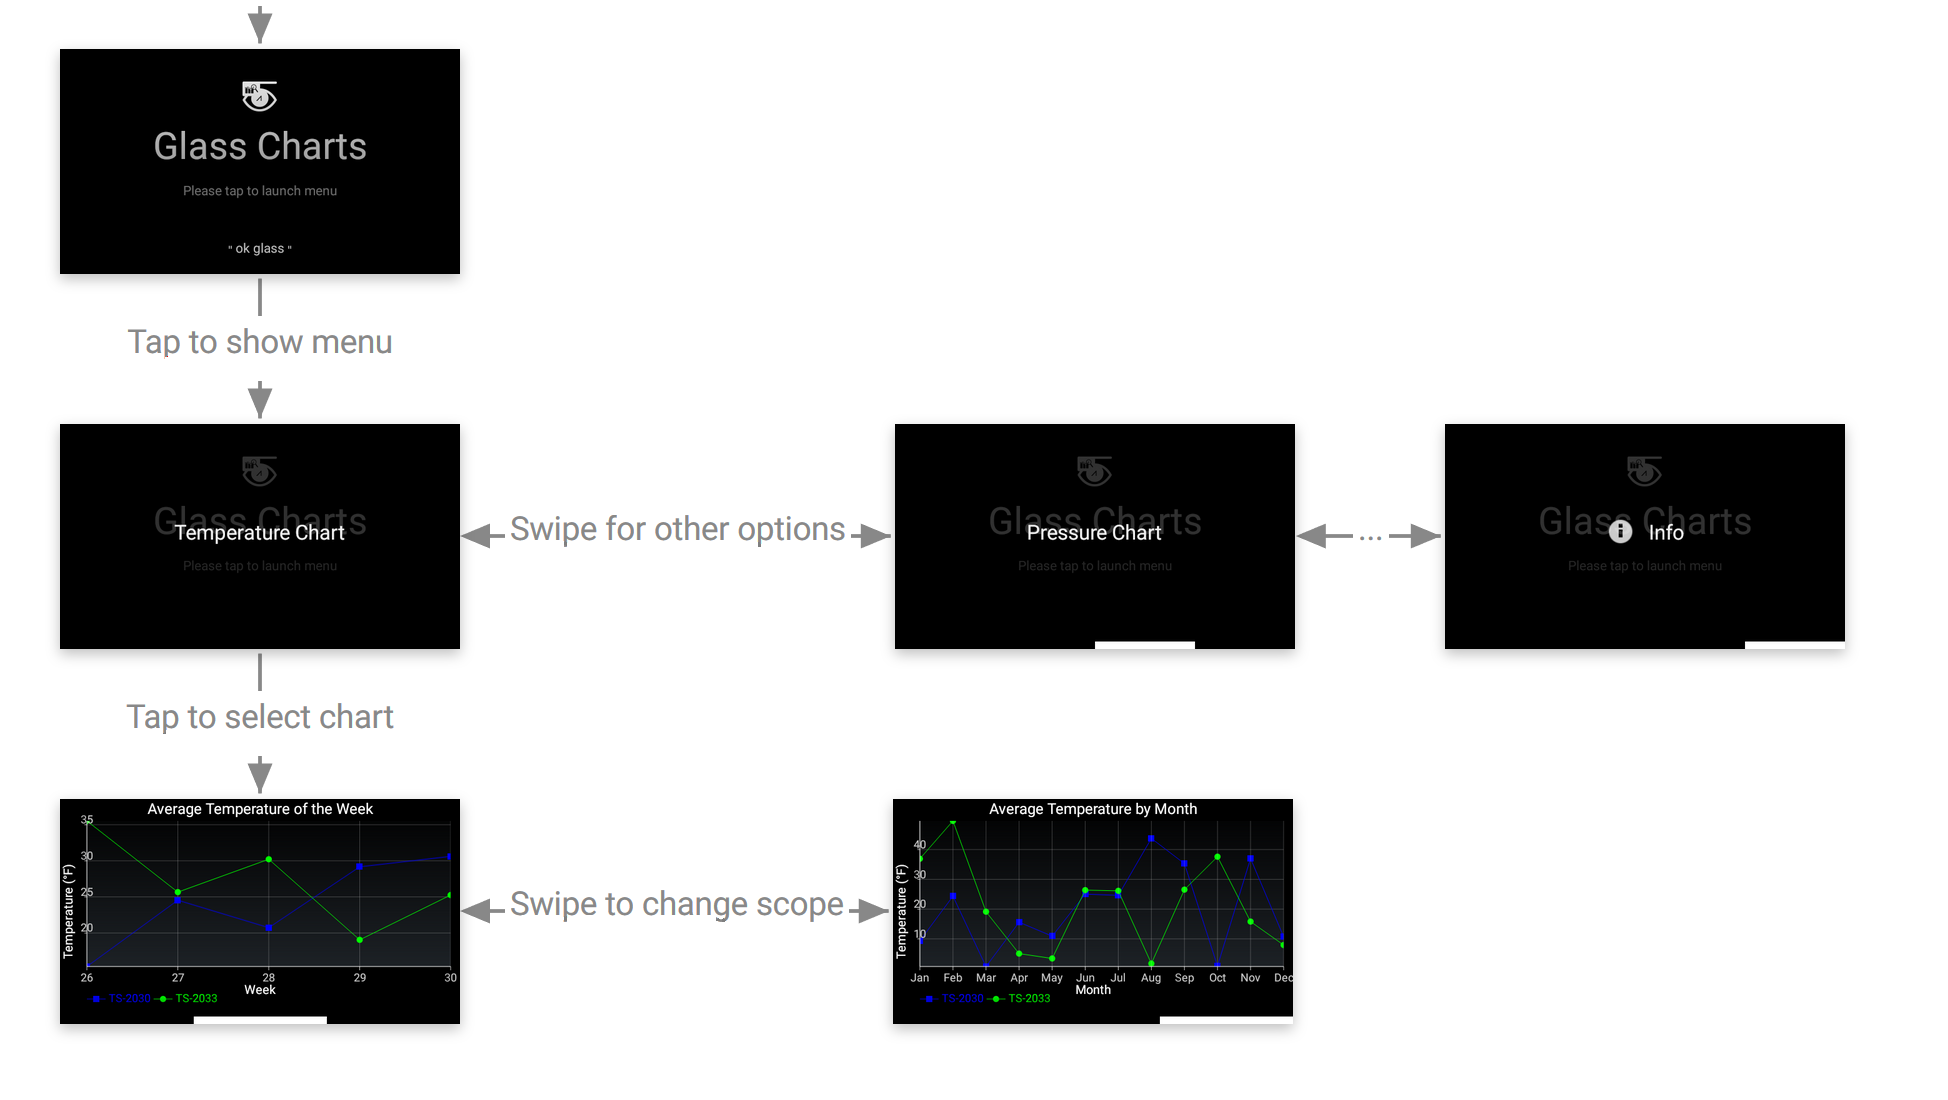
\includegraphics[width = 0.7\linewidth]{images/project_card_flow.png}
\caption{Glass Charts Flow Design}
\label{glassflowdesign}
\end{figure}

Our application has basically 5 card activities, which are the main activity, 3 environmental chart activities (temperature, humidity and pressure) and an instruction activity that shows the basic accepted commands inside each chart, as pictured below.

\begin{figure}[H]
\centering
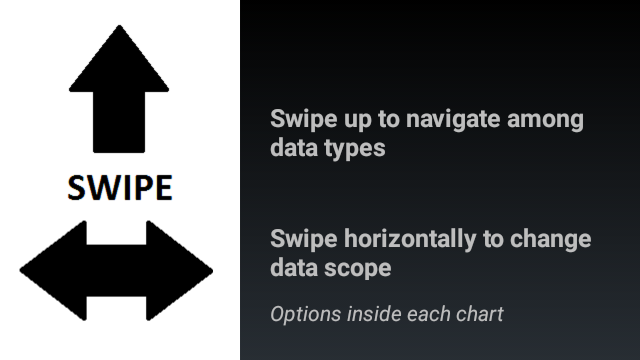
\includegraphics[width = 0.4\linewidth]{images/information_card.png}
\caption{Instruction Card Activity}
\label{instructioncard}
\end{figure}

The images that follows are examples of the charts generated by our application. They show a little bit of what the chart library is capable of presenting.

\begin{figure}[H]
\centering
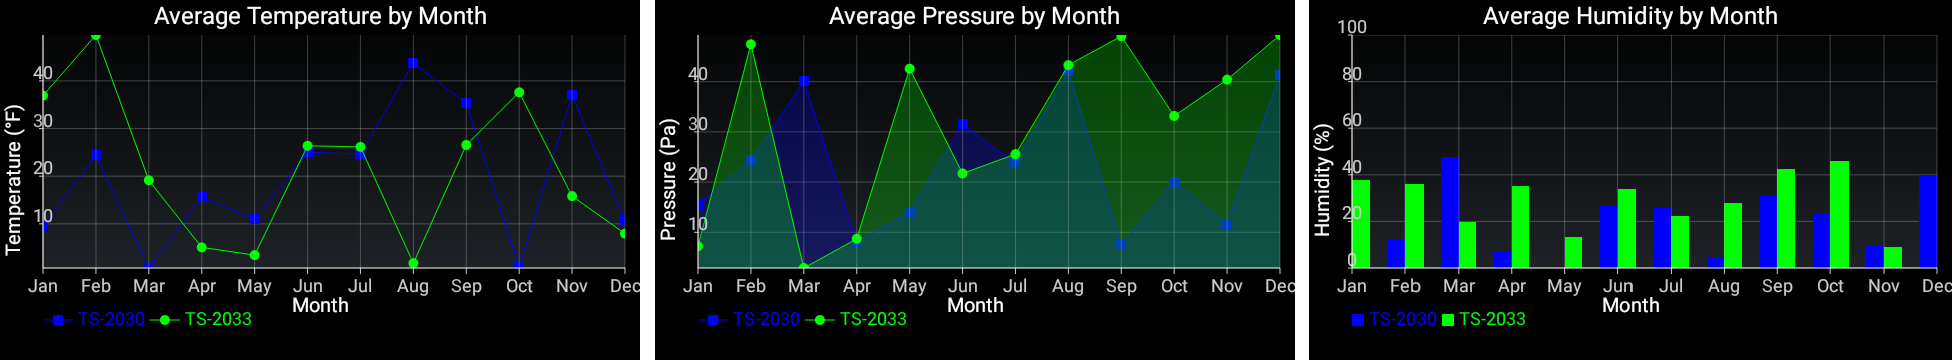
\includegraphics[width = 0.9\linewidth]{images/chart_example.png}
\caption{Example of Charts Generated in our Project}
\label{chartsexample}
\end{figure}

\section{Future Work}

There are some points that could be improved on the project developed. Improvements that could be applied on the application that runs on Google Glass itself \cite{googleglassproject} and also on the server and the database.

Talking about the application running on Google Glass, the implementation of voice commands inside the application to navigate among charts and access different types of data would be something very helpful that would place the application in another notch. Being very important to mention that it would change a lot how the application is used, into a good way.

Another work that could be done is the test of other charting libraries in order to see and evaluate how they perform with the platform and all its limitations. There could be other libraries that perform better than the one used, resulting in a better final experience for the user.

Also, a nice way to improve usability would be adding a geolocation feature, in a way that the application can identify the building the user is in and then display information according to that location.

Referring to the back-end, security is something that could be improved a lot when it comes to the connection that exists among the server, the database and the sensors that are pushing data into the server. An authentication method to check if the device that is pushing data is authorized to do so is something that would be very helpful.

A study about the performance also could be done by comparing if the use of sockets would be a better idea over the HTTP calls that are being used currently. Also, checking how capable the current back-end is to handle a big number of devices and calls is very important in order to have an idea of how reliable it is.

\section{Conclusion}

With the development of this project, it is possible to notice few characteristics related to Google Glass and to the applications that run on it.

To develop to Google Glass is a tough task indeed. As already mentioned in the other sections, such as the difficulties section, there are plenty of reasons that make the development something not that simple. Starting from the community that for being small, can make everything even harder. There are also other reasons like the need of a connection with a smartphone in order to be able to get everything from the capability of the device. 

Even though it is a tough task, developing something for Google Glass is for sure worth it. It is an amazing device with a lot of possibilities and potential. You just need to adapt your needs to what is provided by the platform. The fact of everything being kind of simple in this device does not mean that the it has no power or is useless.

This project is another example, among all the others we already have, of how powerful and helpful this device is. All that is needed is to give it a try.

\section{Acknowledgements}

\begin{figure}[H]
\centering
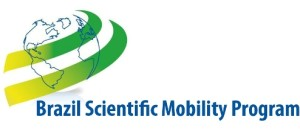
\includegraphics[width = 0.5\linewidth]{images/bsmp_logo.jpg}
\label{bsmp}
\end{figure}

\begin{figure}[H]
\centering
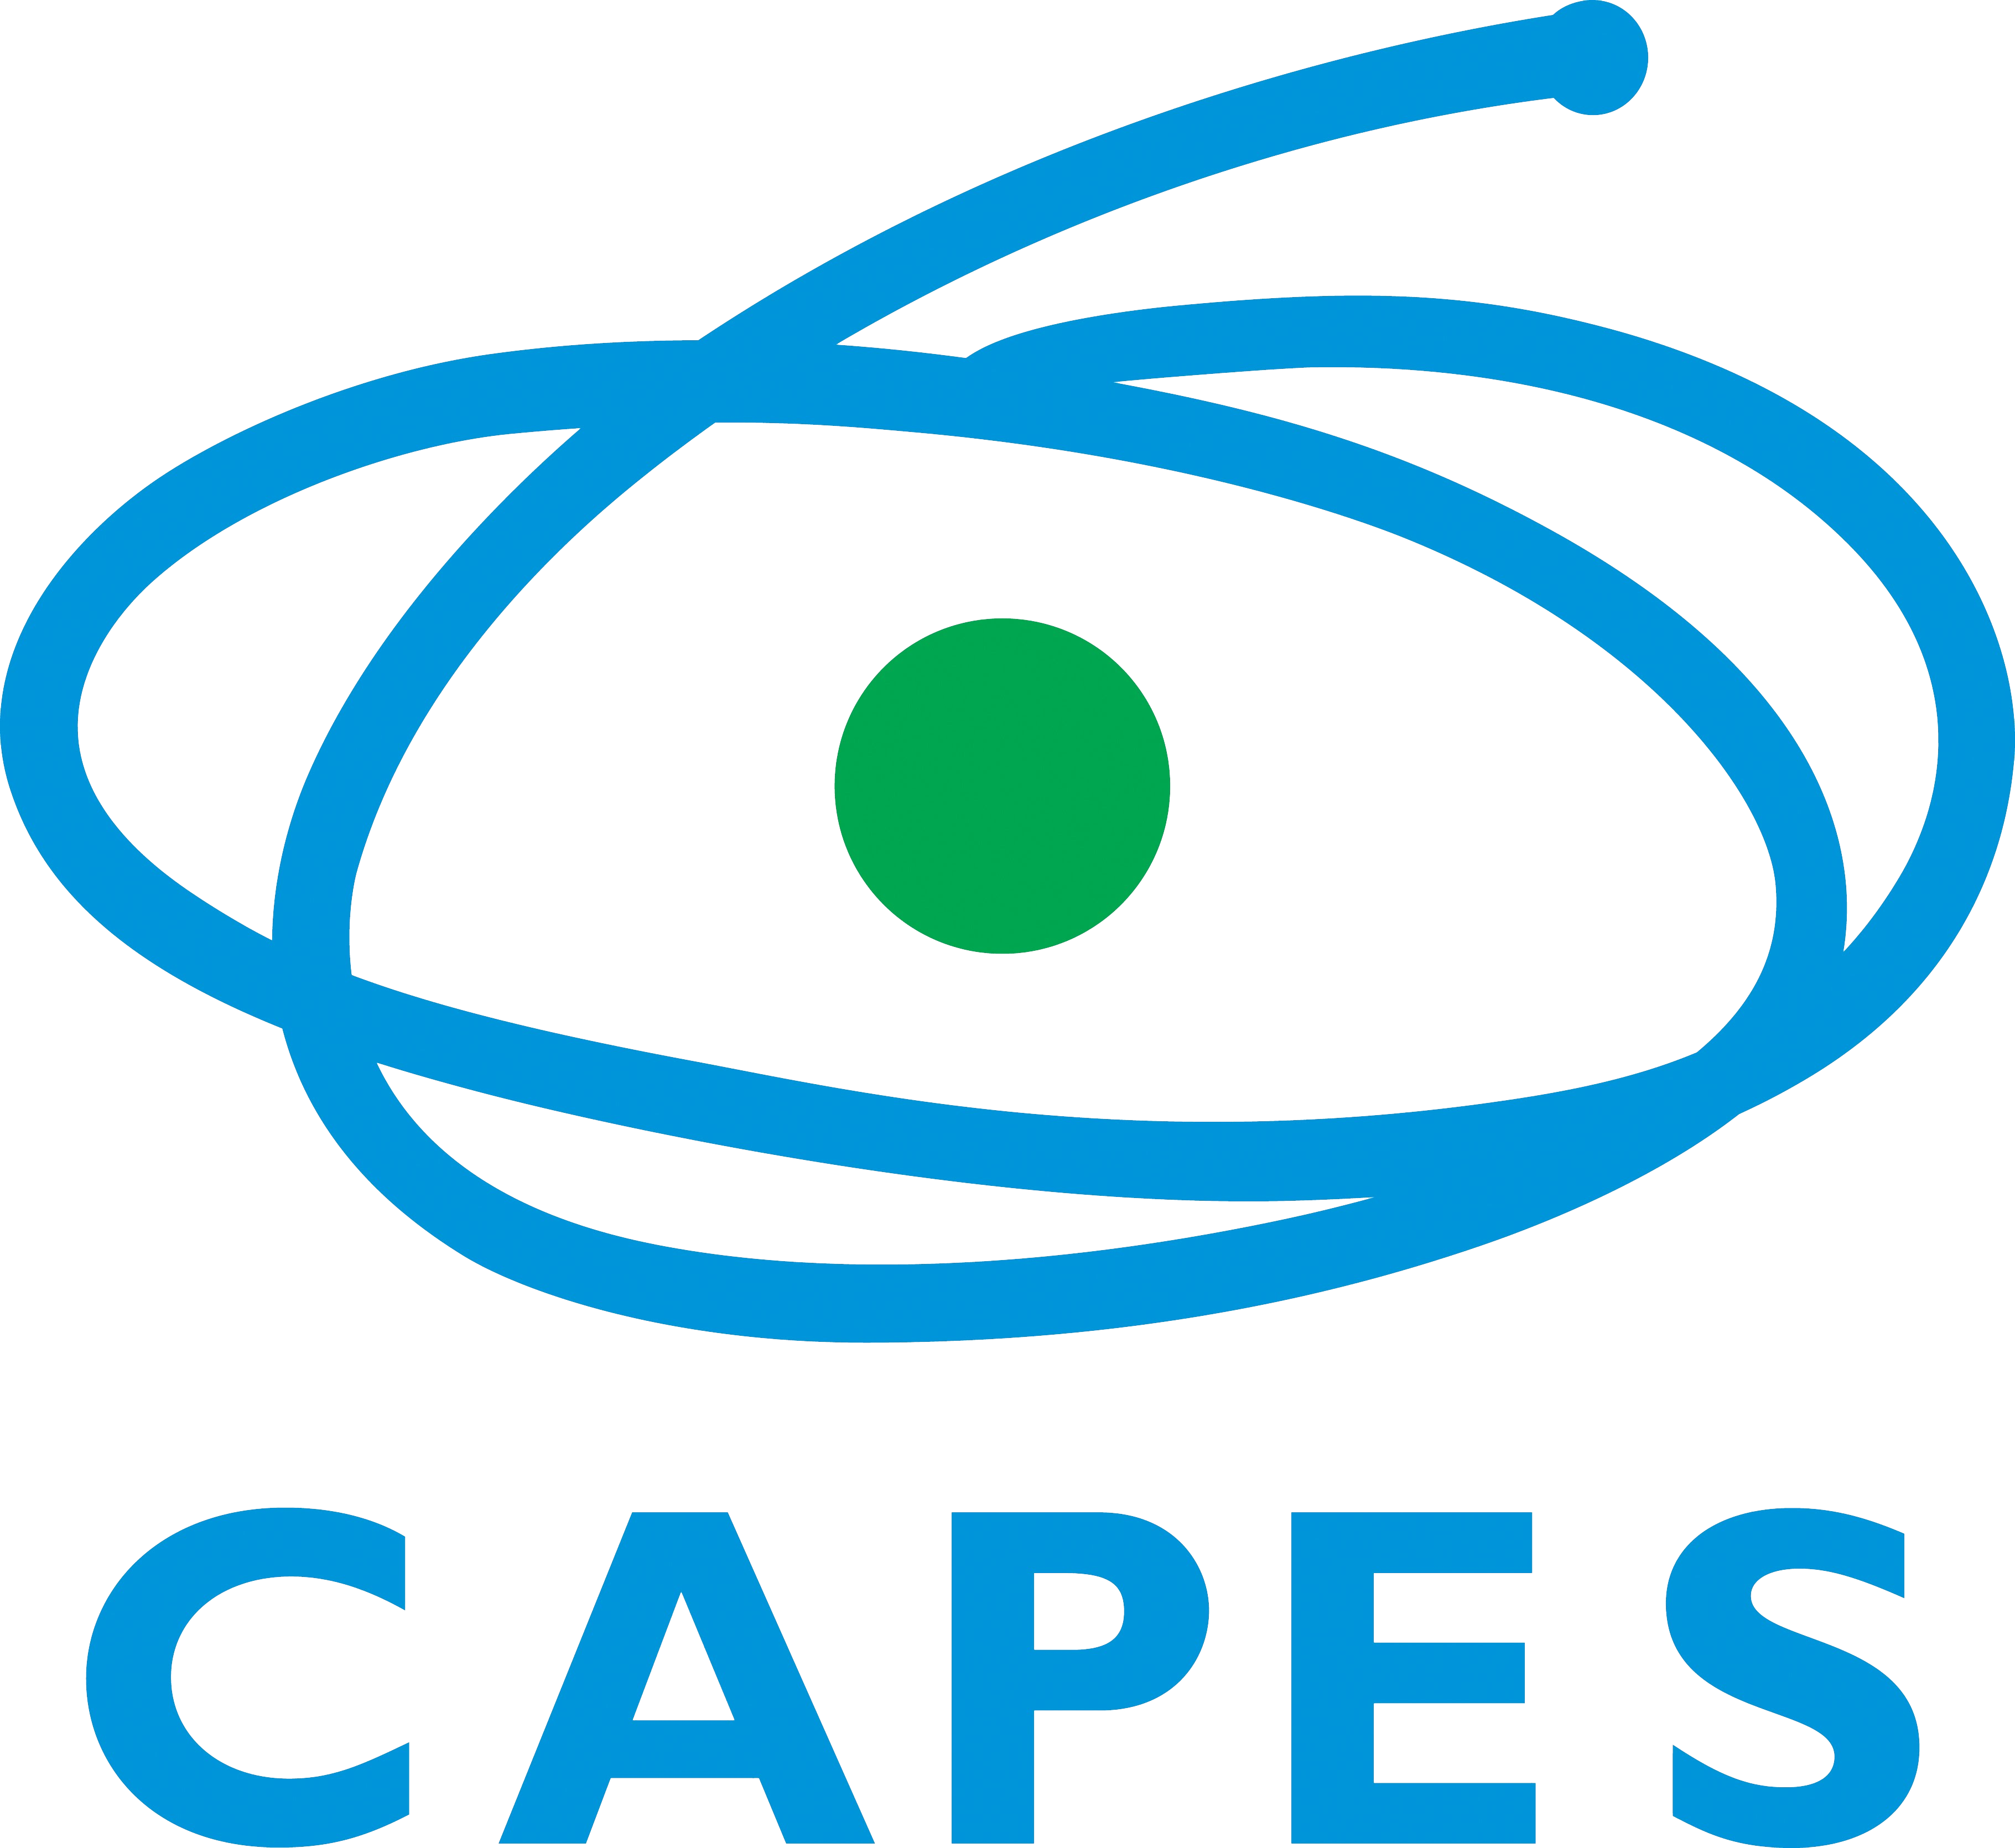
\includegraphics[width = 0.3\linewidth]{images/logo_capes_transparente.png}
\label{capes}
\end{figure}

\medskip    

\begin{figure}[H]
\centering
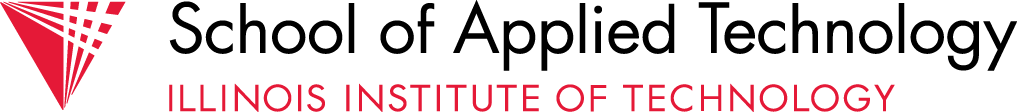
\includegraphics[width = 1.0\linewidth]{images/IIT_SAT_horiz_186_blk.png}
\label{iittech}
\end{figure}

\newpage

\begin{thebibliography}{15}

\bibitem{glassdevelopers} 
Google Glass: Build Glassware that is available at a user's glance on Glass,
\\\texttt{https://developers.google.com/glass/}

\bibitem{androiddevelopers} 
Android Development: Build Beautiful Apps,
\\\texttt{https://developer.android.com/}

\bibitem{tecmundoandroid} 
Tecmundo: Google Glass News,
\\\texttt{http://www.tecmundo.com.br/google-glass}

\bibitem{v8server} 
Chrome V8: Google's high performance, open source, JavaScript engine,
\\\texttt{https://developers.google.com/v8/}

\bibitem{mongodb} 
MongoDB: Building on the Best of Relational with the Innovations of NoSQL,
\\\texttt{https://www.mongodb.com/}

\bibitem{mongodbdocs} 
MongoDB Documentation: Getting Started with MongoDB,
\\\texttt{https://docs.mongodb.com/getting-started/}

\bibitem{heroku} 
Heroku: Setting up, operating and maintaining your own platform,
\\\texttt{https://www.heroku.com/}

\bibitem{herokudev} 
Heroku with Node.js: This tutorial will have you deploying a Node.js app in minutes,
\\\texttt{https://devcenter.heroku.com/articles/getting-started-with-nodejs}

\bibitem{acharengine} 
AChartEngine: Charting library for Android applications,
\\\texttt{https://github.com/ddanny/achartengine/}

\bibitem{git} 
GitHub: how people build software,
\\\texttt{https://github.com/}

\bibitem{googleglassstyle} 
Miller, Claire Cain (February 20, 2013). 
\textit{"Google Searches for Style". }[\textit{"Here’s your chance to get Google glass", Gadget cluster, Apr 2014}].
The New York Times. Retrieved March 5, 2013.
 
\bibitem{googleglassproject} 
Velazco, Chris (April 4, 2012).
\textit{"Google's 'Project Glass' Augmented Reality Glasses Are Real and in Testing".}
TechCrunch. Retrieved April 4, 2012.
 
\bibitem{glassprivacy} 
Arthur, Charles (March 6, 2013).
\textit{"Google Glass: is it a threat to our privacy?".}
The Guardian (London). Retrieved March 7, 2013.
 
\end{thebibliography}

\end{document}
